\textbf{COLUNI 2024 -- Questão 32}\par\medskip Observe o mapa do estado de Roraima.

\begin{center}
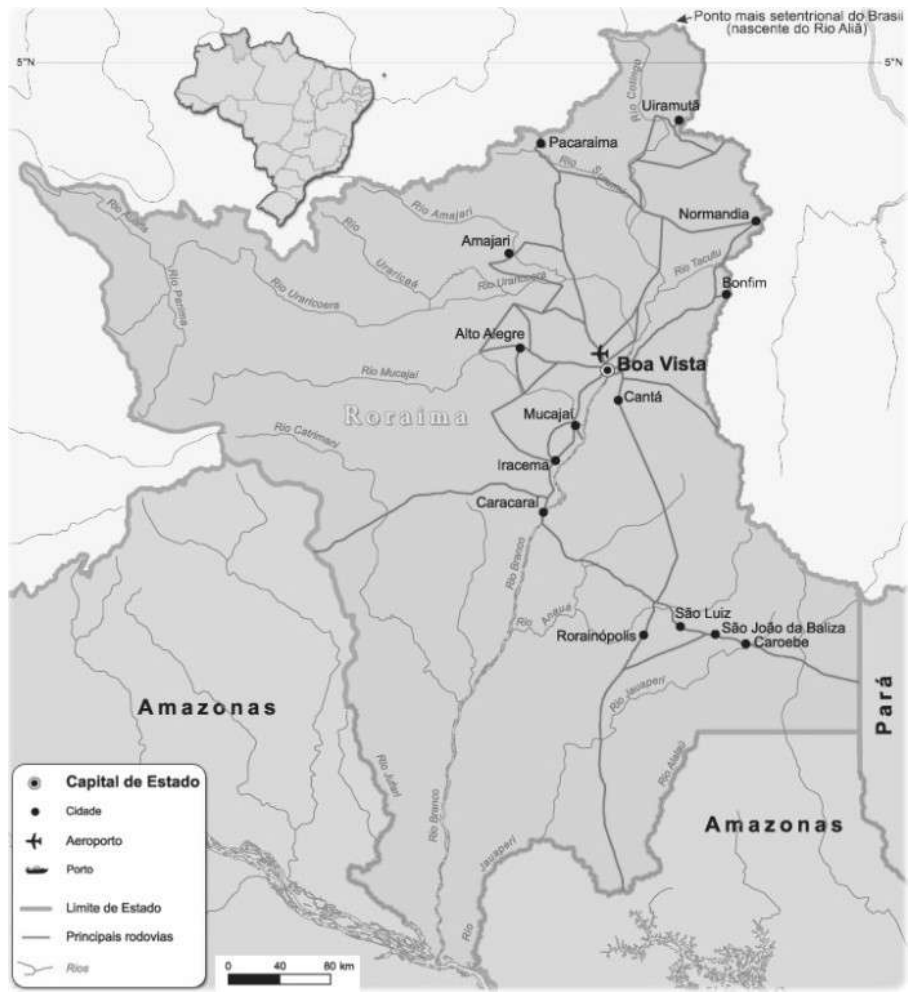
\includegraphics[width=0.72\linewidth]{static/simulados/coluni/figuras/2024/questao-32/figura-1.png}
\end{center}

\begin{center}Fonte: https://www.guiageo.com/roraima.htm. Acesso em: 01 ago. 2023.\end{center}

Considerado o mais setentrional dos estados brasileiros, Roraima é um jovem estado, criado pela Constituição Federal de 1988. Com base na análise do mapa e na divisão regional brasileira, é CORRETO afirmar que:
\begin{enumerate}
\item o estado pertence à Região Norte e sua posição geográfica está totalmente localizada abaixo da linha do
      equador, portanto, no hemisfério sul.
\item a densidade demográfica do estado é extremamente alta, possuindo uma grande concentração
      populacional, apesar de seu povoamento ser recente.
\item o estado de Roraima possui o ponto mais ocidental do país, sendo denominado de Monte Roraima, onde
      se localiza o Pico da Neblina, o mais alto do Brasil.
\item a bacia hidrográfica do estado é típica da Região Norte, com rios em regime pluvial, que correm para o
      oceano e fazem parte da Bacia Amazônica.
\end{enumerate}
